\chapter{Introduction to Stability} %(notes page 65 and 66)
\label{sec:IntroductionToStability}
\index{stability}

Given the models presented in Chapter \ref{sec:ModelingLeggedLocomotion}, we'd like to analyze the dynamics of their motion. Much of the analysis will be to determine the stability of the motion, so it is important to have a good idea of what stability means in this context, before embarking upon these analyses. 

In the context of legged locomotion, a stable system is one that can reject disturbances. In a sense, this defines locomotion. We consider locomotion to be a stable periodic motion of a dynamical system, where the dynamical system is defined by ordinary differential equations and perhaps some collision equations. Locomotion is a stable fixed point on a poincare section. 

A poincare section is...



This can be a really short chapter that simply explains the way the models will be assessed for stability. I recommend writing this after writing the other sections, basically as an explanation of things one should know before reading the other sections. The remainder of this chapter can be a list of resources and topics for those who are interested in more kinds of stability, like Ogata or root locus or Nyquist.

There are a few brief things you should know before we can talk about dynamics in the next chapter.

% FIGURE
\begin{figure}[h]		% h="here" t="top" b="bottom" p="separate page"
\begin{centering}
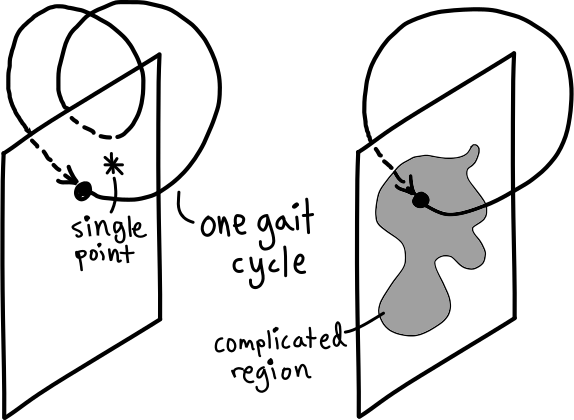
\includegraphics[width=0.5\textwidth]{Figures/Attractors}\par
\end{centering}
\caption{Attractors}
\label{fig:Attractors}
\end{figure}
%

% FIGURE
\begin{figure}[h]		% h="here" t="top" b="bottom" p="separate page"
\begin{centering}
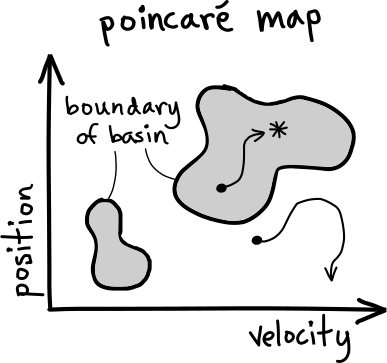
\includegraphics[width=0.3\textwidth]{Figures/BasinOfAttraction}\par
\end{centering}
\caption{BasinOfAttraction}
\label{fig:BasinOfAttraction}
\end{figure}
%

% FIGURE
\begin{figure}[h]		% h="here" t="top" b="bottom" p="separate page"
\begin{centering}
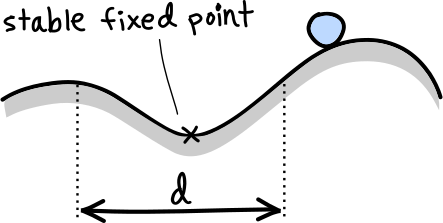
\includegraphics[width=0.5\textwidth]{Figures/BallOnHill}\par
\end{centering}
\caption{BallOnHill}
\label{fig:BallOnHill}
\end{figure}
%

\section{Poincare Sections}
\index{Poincare sections}
